\newpage
\section{Symmetric abstractions}\label{symmetric-abstractions}

% symmetry is cool
Symmetry is a concept from pure mathematics, which has found major success in physics (for example, \href{https://en.wikipedia.org/wiki/Noether%27s_theorem}{see Noether's theorm}).
Symmetry has also had success in machine learning. For example, the formalism has
helped us understand convolutional neural networks (ref), and disentanglement \cite{Higgins2018}.

% also, to disentanglement
% % Connection to causal hierarchy. Cite Pearl. Association, intervention, counterfactuals.
% Also recently noted by \cite{Caselles-Dupre2019}, ... where they assume that
% the group actions are the actions of the RL environment.
% This doesn't really make sense. Also, will miss many symmetries like ???

% occam's razor
% Occam's razor is a core idea behind much of statistics, ML and science. Simple
% hypotheses should be preferred as the are more likely to be right.


\subsubsection{Definition}

We say that an object is symmetric if it has a 'group' structure.

A group is a set, $G$ (\textit{say the set of rotations, $\{0, 90, 180, 270\}$}),
and an operation $\circ$ that combines any two elements $a$ and $b$ to form
another element (\textit{rot $90$ composed with rot $180$ is rot $270$, or} $a \circ b = a + b \;\text{mod} 360$).
To qualify as a group, the set and operation, $(G, \circ)$, must satisfy four requirements;

\begin{itemize}
	\tightlist
	\item \textbf{Closure:} For all $a, b \in G$, the result of the operation $a \circ b$ is also in $G$. (\textit{every composition of two rotations, must also be a rotation})
	\item \textbf{Associativity:} For all $a,b,c \in G$, $(a\circ b) \circ c = a\circ (b\circ c)$. (\textit{???})
	\item \textbf{Identity element:} There exists and element $e\in G$ such that, for every element $a\in G$, the equation $e\circ a = a\circ e = a$ holds. (\textit{there must exist a rotation that doesn't rotate})
	\item \textbf{Inverse element:} For each $a \in G$, there exists an element $b \in G$, commonly denoted $a^{−1}$, such that $a \circ b = b \circ a = e$. (\textit{we must be able to undo any rotation})
\end{itemize}

For example, we can imagine the \textit{action} of this rotation group $\big(0, 90, 180, 270, \circ \big)$ on a playing card. (bad example!?)

\begin{figure}[h!]
	\centering
	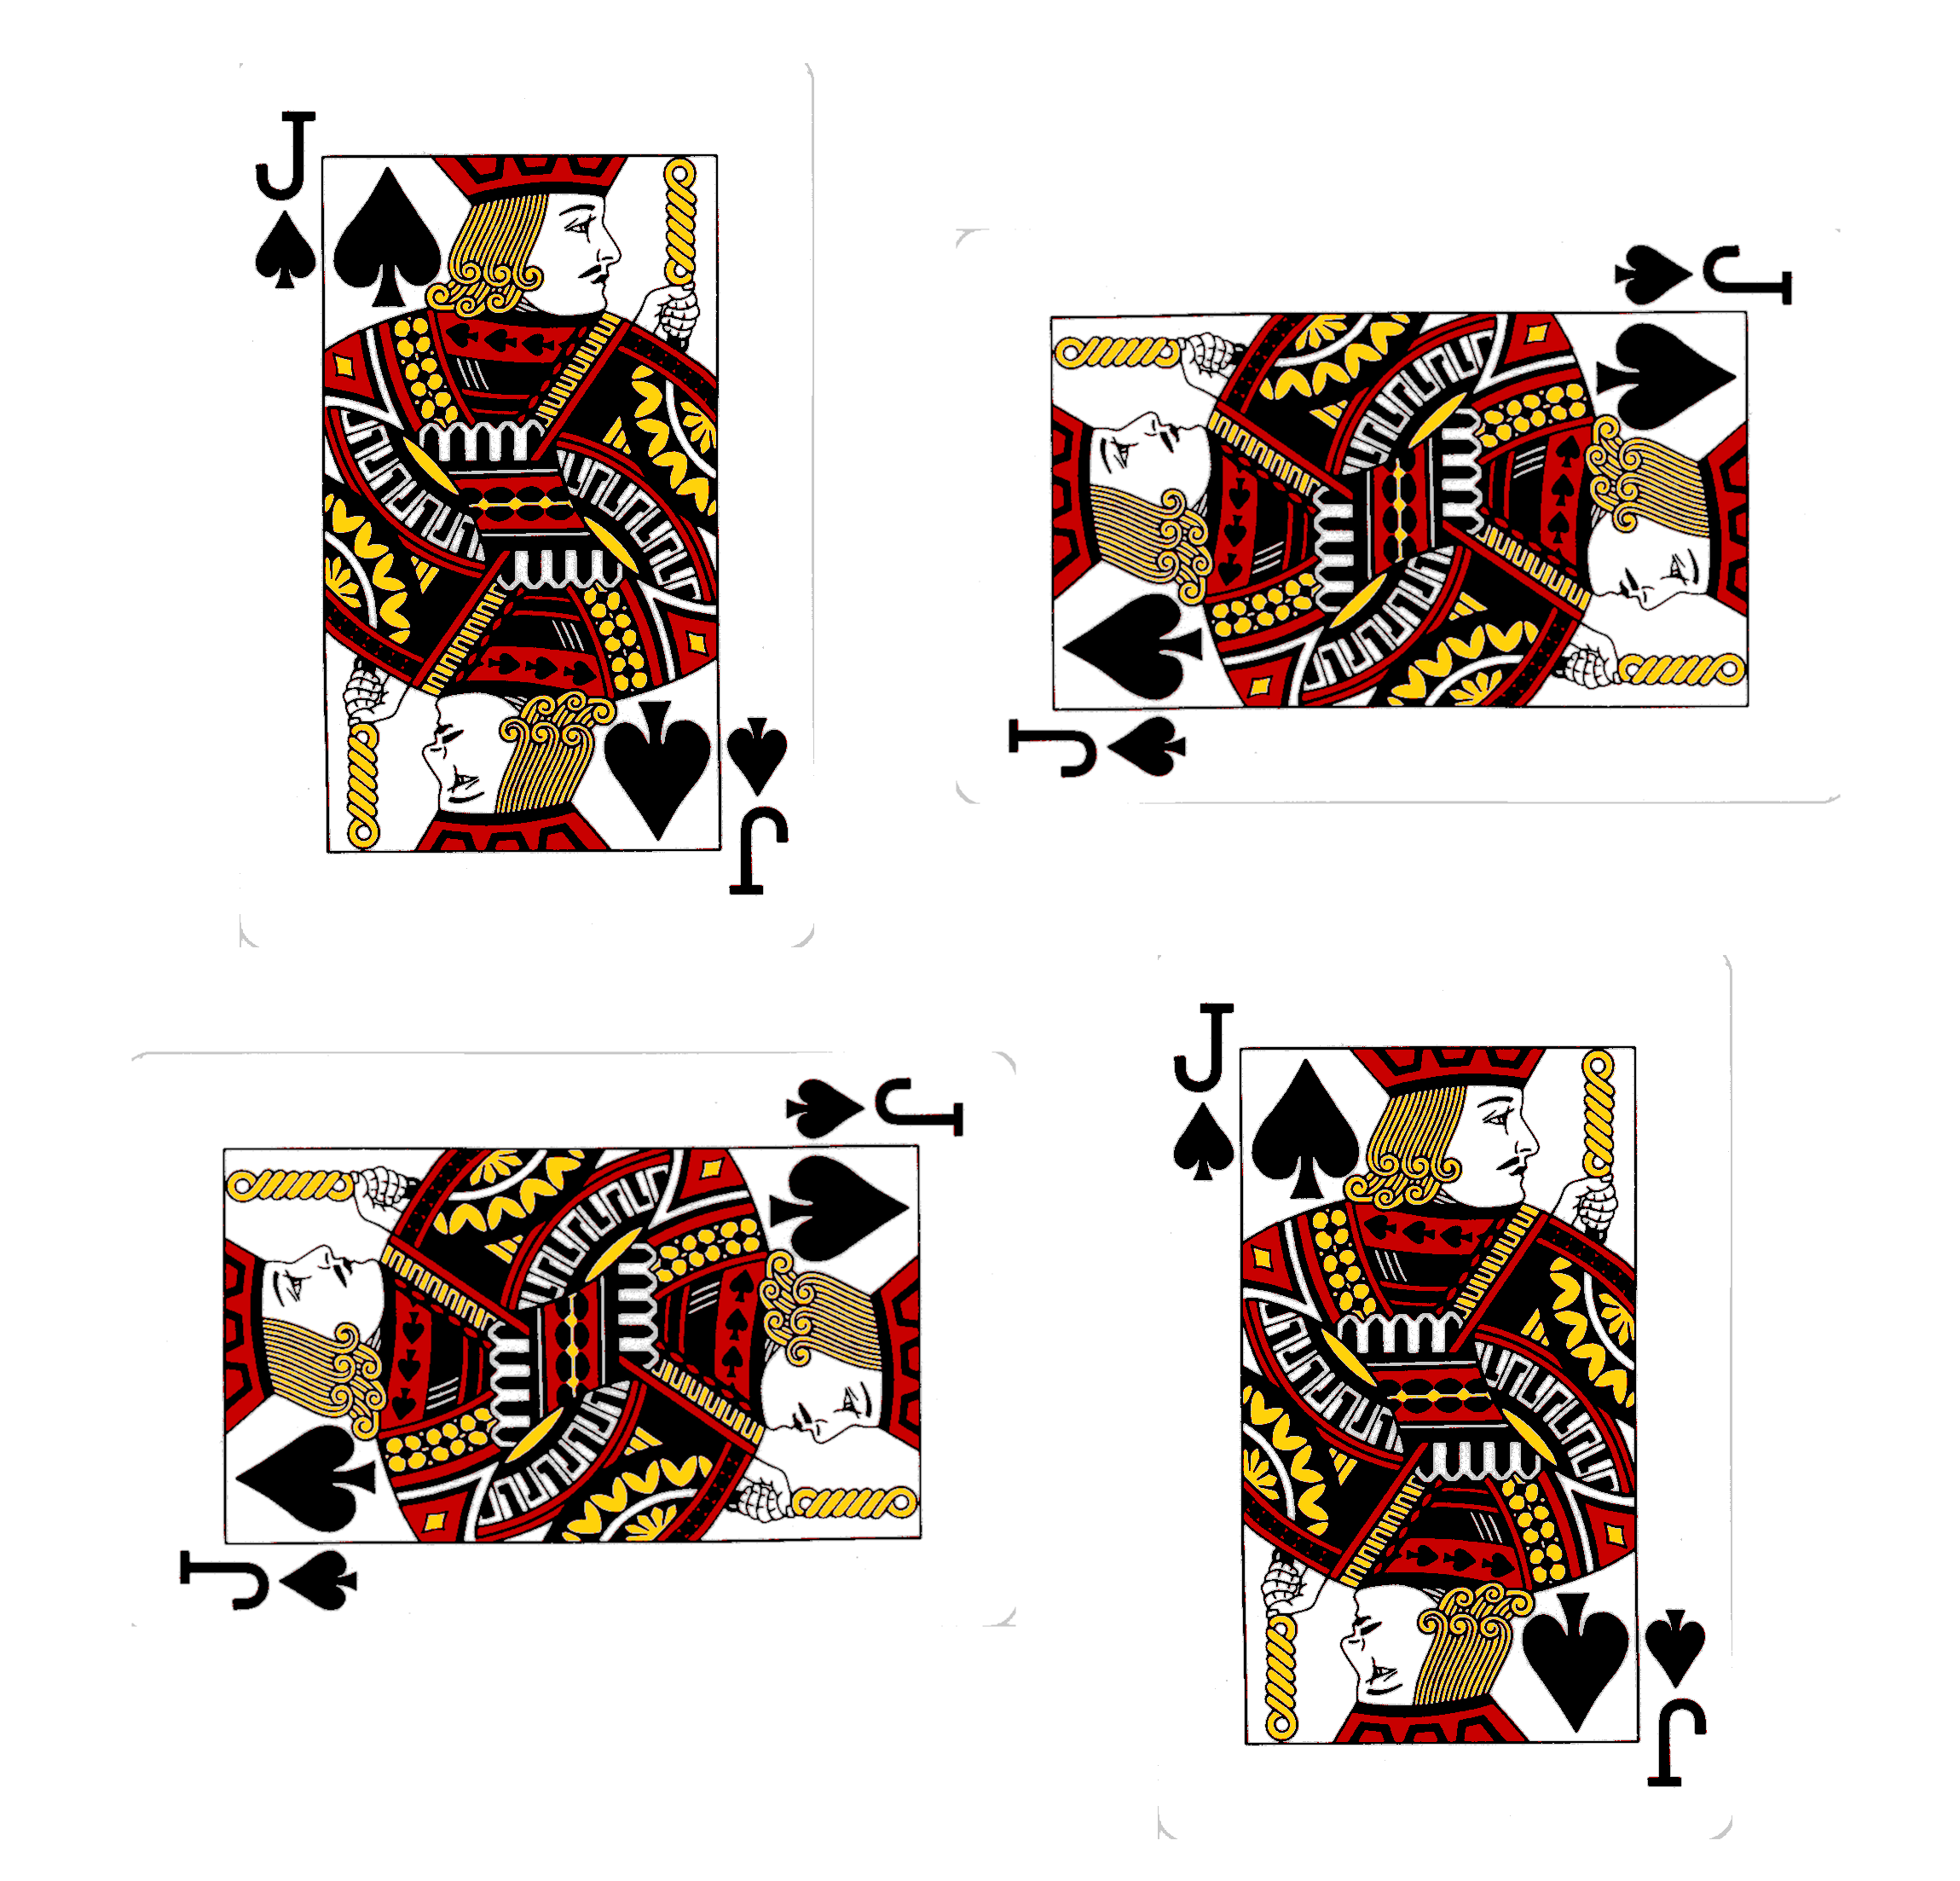
\includegraphics[width=0.75\textwidth,height=0.5\textheight]{../../pictures/images/jacks.png}
	\caption{Here we have applied the group of four rotations to a Jack of spades.
	However, we see that there exists symmetry within the these rotations,
	there are only two distinct rotations, vertical and horizontal. This is because }
\end{figure}

{\color{red}The action of a group on XXX. also. order of a group}
Where $\phi: G \times X \to X$ is a group action. (need to define an action)

\begin{displayquote}
\textsl{How can symmetries be used to build abstractions?}
\end{displayquote}

We can use a group structure to define a similarity (or equivalence relation),
$a \sim_G b$ iff $\exists g \in G: a = g \circ b$. {\color{red} for example??} Therefore, we can use this
 notion of similarity to construct abstractions as we did in \ref{C:abstraction}.

% How does knowing the specific structure of the similarities help?   !!!!!
% If we are just going to group them together?

\subsection{A symmetric inductive bias}

% Following our insights from \ref{symmetry} and \ref{???}.
% This is about generalising using an inductive bias towards symmetry.

In \ref{infer-similarity} we considered using similarities
to build an abstraction. But, learning pairwise similarities does not give
you the ability to generalise. To generalise you need (accurate) priors \cite{Wolpert1996}.

Existing approaches to estimating similarity generalise as the (measure of) similarity encodes priors.
For example;
If our measure of similarity is parameterised as a CNN, then the CNN implicitly encode preference for smooth and local functions. (ref)
If our measure of similarity is trained using SGD, SGD implicitly encodes a preference for low rank solutions (when applied to ???).... ref.

In this section we explore how to construct a prior that says:

\begin{displayquote}
	\textsl{"We believe that the problems we are given are likely to have group structure."}
\end{displayquote}

This symmetric prior allows us to impose abstract structure on potential similarities, without specifying
the 'details' of these similarities.

% \subsubsection{Closedness and generalisation}
%
% The key property we are interested in is the \textit{closure}.
% By requiring the
%
%  Symmetry is a stricter notion of similarity, it requires ...?
%  % If $x, x' \in X$ are symmetric, then there must exist $f$ such that $f(x) = x'$.
%  % Where, $(X, f)$ must satisfy the group axioms, (closure, associativity, identity, inverse).
%
%  Two $x, x'$ are considered symmetric if $\exists g\in G$

% - What about symmetries that are products of subgroups? $S = Z_2 \times Z_3$? Are they easier to infer?
% - Within the same $n$. Is there a notion of more or less complex group structures??
% - Need to show that NNs dont have the right symmetric inductive bias. They dont generalise. !!!

\subsection{A measure of symmetry}

To discover symmetries, we need to be able to measure them.
Therefore, wen need to construct a measure of symmetry, $S: X \to \mathbb [0, 1]$, that returns higher values for 'more' symmetric objects.
We hope to use this measure to bias a learner towards more symmetric guesses (see \ref{thomspon-sampling}).

Given some object, $x \in X$, we want to know, how symmetric is that object?
But, what makes something more or less symmetric?
We define the amount of symmetry to be: the order of the largest group that $x$ is invariant to.

For example, $x_{ab} = [a,a,b,b]$ should be considered more symmetric than $x_{abc} = [a,a,b,c]$ because,
$x_{ab}$ is invariant to actions of $S_2 \times S_2$, while $x_{abc}$ is only invariant to actions of $S_2$.
{\color{red}Do i need to show this?!? need to explain properly}

Note, the larger the group order, the coarser the abstraction we can build. We can group together $x_{ab}[0] \sim x_{ab}[2], x_{ab}[1] \sim x_{ab}[3]$, thus building an abstraction of size $2$.
{\color{red}Should show it is coarser in a formal sense...}

% This, makes sense as we can build coarser abstractions from the groups of higher order.
% So by preferring groups of higher order, we are able to build coarser abstractions.

We write this measure of symmetry as;

\begin{align*}
G^{* } &= \mathop{\text{max}}_G |G| \tag{pick the largest group}\\
\text{s.t.} \;\; &\forall g\in G, x = \phi(g, x) \tag{that $x$ is invariant to} \\
S(x) &= e^{n-|G^{* }|}
\end{align*}

While this measure of symmetry captures some of what we want, it does not work on inputs of interest.
It only considers exact symmetries.

\subsubsection{Approximate symmetries}

Our intuition tells us that $x = [1,1.001,2,2]$ is close to being as symmetric as
$x = [1,1,2,2]$. So rather than asking: \textit{is $x$ invariant to $G$?}, we can ask
\textit{How close is $x$ to being invariant to $G$?} We can write this as;

% The fundamental complexity of the nearest symmetry, and the distance between that symmetry an

\begin{align*}
C(x) &= \mathop{\text{min}}_G \sum_{g_i\in G}\parallel x-\phi(g_i, x)\parallel_2 - \beta |G|\\
S(x) &= e^{-C(x)}
\end{align*}

% What about characterising the complexity by the number of generators /relations.
% Or something information theoretic?

\subsubsection{Implementation issues}

The approximate measure of symmetry defined has two computational issues.

\begin{itemize}
	\tightlist
	\item The search over groups. There are too many groups to enumerate. How can we rationally search through them?
	\item The possible actions of a group on $x$. Grow with !??!.
\end{itemize}

Say $X$ is a subset of $\mathbb R^n$. Then there are $n!$ possible group elements, each corresponding to a permutation.



\paragraph{The number of possible groups}

Constructing the possible groups. The naive method, of generating all the permutations, and checking, which combinations of those permutations is closed requires ???.  $\mathcal O(n! \times n!)$

Alternatively, it may be possible to build up from smaller symmetries!? TODO...

\paragraph{The number of possible actions}

The number of possible actions grows quickly. Consider the possible actions of the $S_n$ groups.
In the table below, the rows represent the different $n$. The columns represent $x$s of different dimension.
We count the number of .

No. These are wrong... These are not n of possible actions of $S_n$.

\begin{changemargin}{-3cm}{-3cm}
  \begin{center}
    \begin{tabular}{ c || c | c | c | c | c | c | c | c | c }
        & 2 & 3 & 4 & 5  & 6   & 7   & 8   & 9 & 10 \\ \hline \hline
      1 & 1 & 3 & 6 & 10 & 15  & 21  & 28  & 36   & 45\\ \hline
      2 & 0 & 0 & 3 & 15 & 45  & 105 & 210 & 378  & 630 \\ \hline
			3 & 0 & 0 & 0 & 0  & 15  & 105 & 420 & 1260 & 2150 \\
    \end{tabular}
  \end{center}
\end{changemargin}

And number of actions of $S_2$ are (aka 1-gram swaps). $n_{\text{actions}} = \frac{d}{2}(d-1)$. (for even $n$).


\begin{center}\rule{0.5\linewidth}{\linethickness}\end{center}

For this reason, we start with a restricted family of groups:
groups, whose order can be identified by the existence of a permutation, and ???.

We use a family of permutations that are idempotent. Groups that 'flip' / 'reflect'.
This family of includes any n-wise swap.

Not clear which groups this includes? Symmetric groups, cyclic groups, dihedral????

Why so expensive?!! There is no structure in the states. They are discrete and unrelated.
(at least our representation of them). Cyclic symmetry is easy to detect in (example) because
we ... .

% Alternatively, we could???
% \begin{itemize}
% 	\item Iterate through groups.
% 	\item Iterate through possible group elements, then regularise to be closed.
% 	\item ???
% \end{itemize}

We can construct (and identify) the family of groups $S_{2\times n}$.
If group element $?!?!$ exists, then ...?!

The existence of 2-gram swaps implies $S_2 \times S_2$, see \ref{s2-lemma} for proof.
Similarity, existence of n-gram swaps implies $S_2 \times S_2$.

\subsubsection{Topology}

\begin{displayquote}
\textsl{Let's try to understand this measure we have constructed. How does it behave?
Does it give us the properties we wanted?}
\end{displayquote}

No explicit knowledge of a symmetry. But, a family of symmetries. A higher level prior.!!!

We can see that the measure is invariant to changes in norm.

Properties this measure of symmetry should satisfy are, \ref{}, \ref{}, \ref{}.

\begin{itemize}
	\tightlist
	% \item A symmetry is less complex if it has more 'structure'. Where it can be build via the direct product of subgroups $\mathcal S(C_4) > \mathcal S(C_2 \oplus C_2)$
	% \item Groups that are commutative are less complex $\mathcal S(D_4) > \mathcal S(C_8)$ (because $D_4$ is not abelian)
	\item Symmetries with larger
	\item $\mathcal S([a,a,b,c]) = \mathcal S(10 \times [a,a,b,c])$
	\item An exact group structure should have higher symmetry than an approximate group structure $\mathcal S(([a,a,b,c]) < \mathcal S([a,a+\epsilon,b,c])$
\end{itemize}

\begin{figure}[h!]
\centering
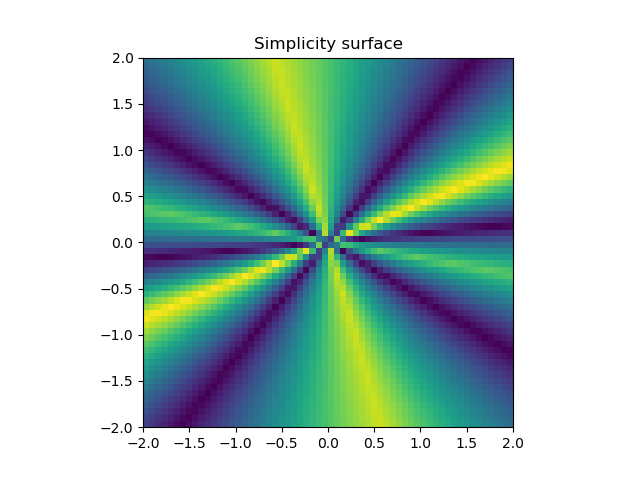
\includegraphics[width=0.7\textwidth,height=0.35\textheight]{../../pictures/figures/complexity_surface_nd-3d.png}
\caption{}
\end{figure}

\begin{figure}[h!]
\centering
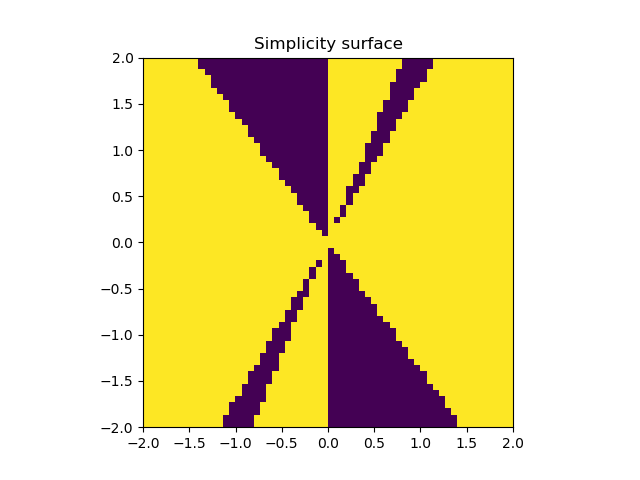
\includegraphics[width=0.7\textwidth,height=0.35\textheight]{../../pictures/figures/complexity_surface_nd-4d-S-0.png}
\caption{A visualisation of our measure of symmetry applied to four dimensional vectors.
We have randomly picked a linear projection from the four dimension, to two dimensions.
Each pixel represents a vector in the 4D space. Lighter color is more symmetric.}
\end{figure}

% \begin{figure}[h!]
% \centering
% 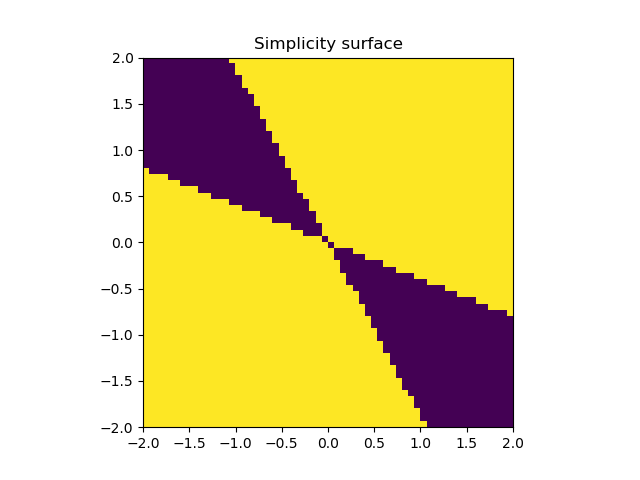
\includegraphics[width=0.7\textwidth,height=0.35\textheight]{../../pictures/figures/complexity_surface_nd-4d-S-2.png}
% \caption{}
% \end{figure}

\subsubsection{Symmetric Rejection Sampling}\label{rejection-sampling}
{\color{red}Should be in the appendix??}
\begin{displayquote}
	\textit{How can we use this measure of symmetry as a prior?}
\end{displayquote}

We can use rejection sampling to bias produce distributions biased towards symmetric samples. Let's see how.

Rejection sampling allows you to generate samples from a target distribution, $p(\cdot)$ (which we cannot efficiently sample from) and a (related) distribution that we can easily sample from, $q(\cdot)$.
$k = \mathop{\text{max}}_x \frac{p(x)}{q(x)} $

{\color{red}Give some intuition about how rejection sampling works.}

\begin{algorithm}
	\caption{Rejection sampling}
	\begin{algorithmic}[1]

		\Procedure{RS}{$p, q, k$}
		\State $t=0$
		\While{not accepted}
			\State $x\sim U([0, 1])$
			\If{$x < \frac{p(x)}{kq(x)}$}
				\State $Break$
			\EndIf
			\State $t += 1$
		\EndWhile
		\State \algorithmicreturn{ $x$}
		\EndProcedure

	\end{algorithmic}
\end{algorithm}

We might have some belief over parameters values $\theta$, given some data, $D_t$, which we write as $p(\theta| D_t)$ (the posterior).
We might also have a prior about likely parameter values, in this case, our belief that they should be symmetric $P_{\text{sym}}(\theta)$. Therefore, we can construct a target distribution using Bayes rule.

\begin{align*}
q(\theta | D_t) = \frac{p(D_t | \theta)P_{\text{sym}}(\theta)}{p(D_t)}
\end{align*}

Thus we have a distribution over parameters, $q(\theta | D_t)$, which we can optimise using maximum a posteriori.

Fortunately, we don't need to construct $P_{\text{sym}}(\theta)$, we only need an unnormalised function that it is proprtional to ({\color{red}ref!!}). Meaning, we can use $P_{\text{sym}}(\theta)\to S(x)$.

Consider an example, we might have some estimate of a parameter's value, $\mu, \sigma$, which follows a gaussian distribution $p(\cdot)$. But, we believe the parameters should be symmetric. Therefore, we can construct a new distribution, $q(x | D_t) = p(\mu, \sigma| x)S(x)$. We can use rejection sampling to generate samples from $q(x | D_t)$.

\begin{figure}[h!]
  \centering
  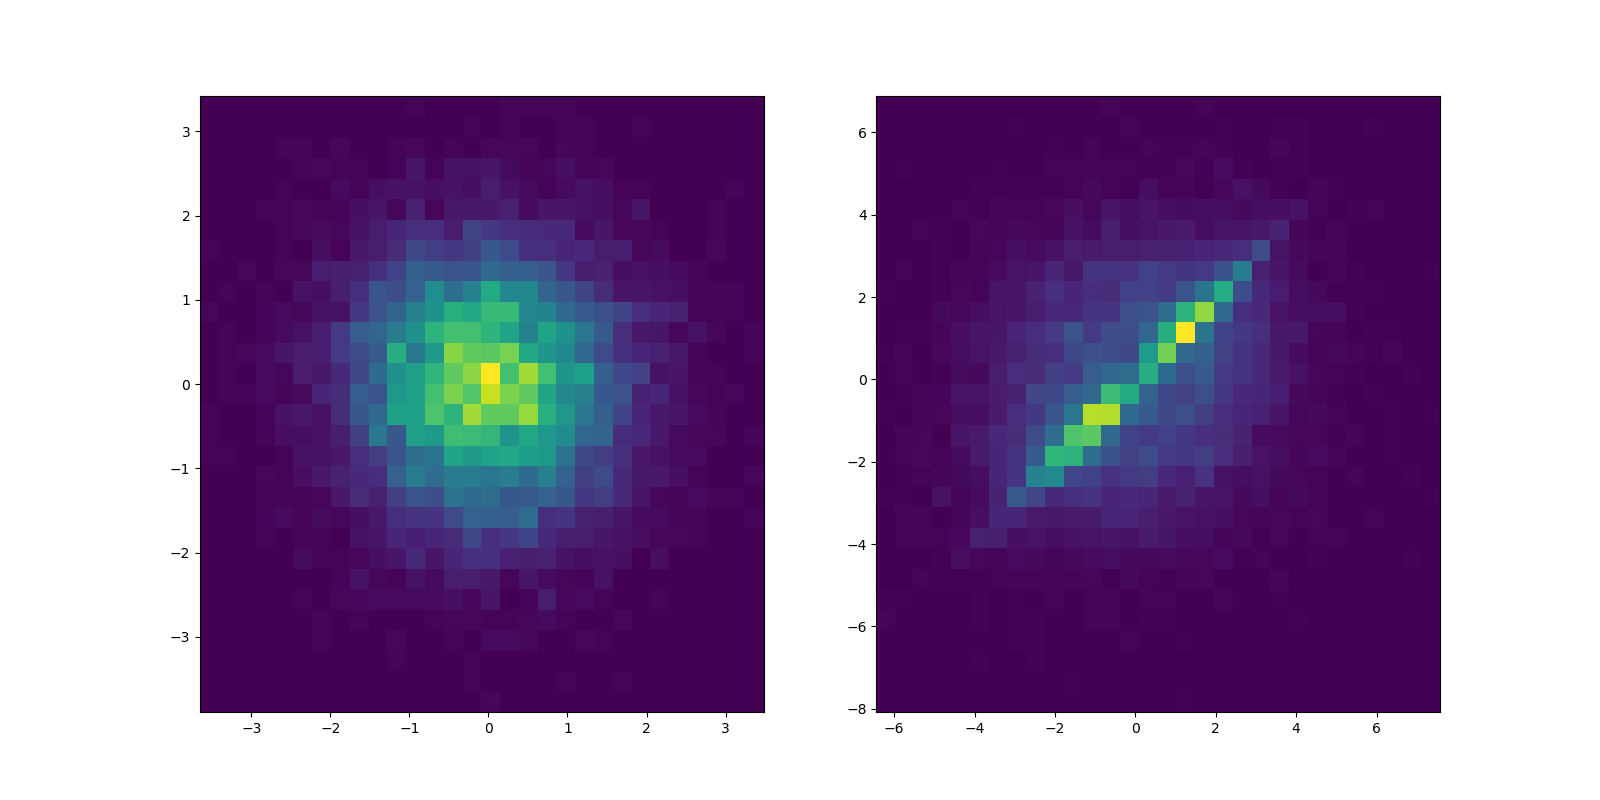
\includegraphics[width=1\textwidth,height=0.25\textheight]{../../pictures/figures/symmetric-gaussian.png}
  \caption{On the left we can see a Gaussian distribution of mean zero and variance one.
  On the right, we have used rejection sampling, with $p(x)$ a gaussian
  distribution augmented by our measure of symmetry, and $q(x)$ being the original gaussian distribution.}
\end{figure}

{\color{red}TODO cut white space from ims}

\begin{figure}[h!]
  \centering
  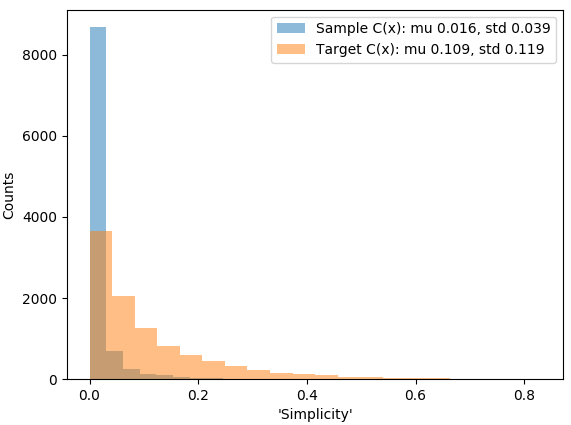
\includegraphics[width=0.8\textwidth,height=0.4\textheight]{../../pictures/figures/s2-prior-rejection-8d.png}
  \caption{Here we have samples from the 'sample distribution', $p(x)$, and the 'target distribution', $q(x)$.
	We can see that the rejection sampling with the symmetry augmented target distrubtion was successful in producing, on average, more symmetric samples. }
\end{figure}


These results really just confirm that we have implemented
rejection sampling correctly, and it works as expected.

% \begin{figure}[h!]
% \centering
% 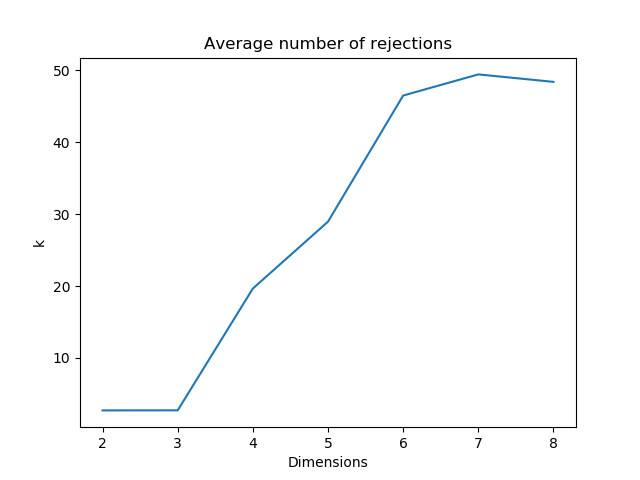
\includegraphics[width=1\textwidth,height=0.5\textheight]{../../pictures/figures/ks.png}
% \caption{}
% \end{figure}

In theory, we use this approach to bias any distribution of our choice to be more symmetric.
However, computational costs.

\subsubsection{Computational issues}

Proximity to symmetric states. How does this change as d increases?

\begin{itemize}
	\tightlist
	\item k as n increases?
	\item k as |G| increases?
	\item Cost to construct |G|?
\end{itemize}

Most general way of adding a prior!?!?
Doesnt assume that SGD is being done, or some parameterisation... !??!?!
Because of that, it's also expensive...

\subsection{Biased Thompson Sampling} \label{thompson-sampling}

\begin{displayquote}
\textsl{We have a way to apply a symmetric prior to a distribution.
How can we use that to make RL more efficient?}
\end{displayquote}

Here we consider how to use a symmetric prior to make Thompson sampling more sample efficient.

\subsubsection{Thompson sampling} \label{ts}
\begin{displayquote}
	\textsl{What is Thompson Sampling?}
\end{displayquote}

\begin{displayquote}
	\textit{Thompson sampling is an algorithm for online decision problems where actions are taken sequentially in a manner that
must balance between exploiting what is known to maximize immediate performance and investing to accumulate
new information that may improve future performance.}\cite{Russo2017}
\end{displayquote}

Less cryptically, Thomspon sampling estimates the model. We then act optimally with respect to the estimated model. However, the estimate uncertainty, so ...? We can write this as follows.

\begin{algorithm}
	\caption{Thompson Sampling}
	\begin{algorithmic}[1]

		\Procedure{TS}{$\gamma$}
		\State $t=0$
		\While{not converged}
		\State $(s, a, r, s')$ \Comment{Observe}
		\State $H_t \leftarrow (s, a, r, s', a')$ \Comment{Update history}
		\State $\tau, R \sim P(\cdot | H_t)$ \Comment{Sample a model}
		\State $Q_{t+1}(s, a) = R(s, a) + \gamma \tau(s'| s, a) Q_t(s', a')$ \Comment{Bellman operator}
		\State $\pi_t = \text{greedy}(Q_{t+1})$ \Comment{Act greedily}
		\State $t += 1$

		\EndWhile
		\State \algorithmicreturn{ $\pi_t$}
		\EndProcedure

	\end{algorithmic}
\end{algorithm}

Where $H_t$ is the history of observations, $\{(s_i, a_i, r_i, s_i') : \forall i \in [0, t]\}$.
And we construct the estimate of the model as independent distributions of the transition and reward functions $P(\tau, R | H_t) = P(\tau | H_t) \cdot P(R | H_t)$. Where $P(\tau | H_t)$
is modelled as the normalised state transition counts {\color{red}should formally define?}.
And $P(R | H_t)$ is modelled as a isotropic gaussian.
These can be estimated by storing state-action-state transition counts
and the incremental mean and variance of the rewards. {\color{red}should give more details?}

Note that we act greedily with respect to the $Q$ function. Normally, this would
lead to sub optimal behaviour, because no exploration is being done. But, Thompson sampling
directs exploration through its uncertainty in the model, $\tau, r$. Thus,
exploration occurs by acting greedily with respect to a sampled model.

% \subsubsection{Abstracted Thompson Sampling}
%
% There may be structure in the model,
% Thompson sampling from estimates of similarity / symmetry.
%
% The likelihood of an abstraction, $P(A|H_t)$, is modelled as a isotropic (actually should really use full covar?!?!) guassian.
%
% \begin{align*}
% 	P(A|H_t) &= \mathcal N(\chi_{\mu}, \chi_{\sigma}) \\
% 	\chi_{\mu} &= \frac{1}{t}\sum_{i=0}^t Q_i \tag{mean} \\
% 	\chi_{\sigma} &= \sqrt{\sum_{i=0}^t (Q_i - \chi_{\mu})^2} \tag{standard deviation}
% \end{align*}
%
% When notice that two states are similar, we group them together. After grouping them, we can apply the Bellman optimality operator.
%
% \begin{algorithm}
% 	\caption{Abstracted Thompson sampling}
% 	\begin{algorithmic}[1]
%
% 		\Procedure{ATS}{$\gamma$}
% 		\State $t=0$
% 		\While{not converged}
% 		\State $(s, a, r, s')$ \Comment{Observe}
% 		\State $H_t \leftarrow (s, a, r, s', a')$ \Comment{Update history}
% 		\State $\tau, R \sim P(\cdot | H_t)$ \Comment{Sample a model}
% 		\State $A \sim P(\cdot | H_t)$ \Comment{Sample a state abstraction}
% 		\State $\tilde \tau, \tilde r, \tilde Q_t = A(\tau, r, Q_t)$ \Comment{Do a model reduction}
% 		\State $\tilde Q_{t+1}(s, a) = \tilde r(s, a) + \gamma \tilde \tau(s'| s, a) \tilde Q_t(s', a')$ \Comment{Bellman operator}
% 		\State $Q_{t+1} = S^{-1}(\tilde Q_{t+1})$ \Comment{Lift the values}
% 		\State $\pi_t = \text{greedy}(Q_{t+1})$ \Comment{Act greedily}
% 		\State $t += 1$
%
% 		\EndWhile
% 		\State \algorithmicreturn{ $\pi_t$}
% 		\EndProcedure
%
% 	\end{algorithmic}
% \end{algorithm}
%
% % if we were certain enough, we could throw away estimates of certain states. and just work in the abstracted domain?!
%
% This doesnt really work. For a few reasons. Costs a lot of keep track of the pairwise state similarities.
% Saves compute on Bellman step.
% But overall, is costs more compute than has been gained.
%
% Shouldn't effect sample efficiency. (unless we replace the tabular model with something that can generalise)

\subsubsection{Biased Thompson Sampling}\label{bts}

\begin{displayquote}
\textsl{Given uncertainty, prefer symmetry}
\end{displayquote}

The difference between \textit{Thompson Sampling} and \textit{Biased Thompson Sampling}
is how we construct the distribution over models, $P(\tau, R |D)$.

We believe that the states will have group structure, a symmetry. ({\color{red}why?})
We use the symmetric rejection sampling method, outlined above (\ref{rejection-sampling}) to bias the
distribution over models towards more symmetric models.

To simplify, we estimate $P_{\text{sym}}(\tau, R)$ as $P_{\text{sym}}(R)$. That is, we believe there will be symmetries in the reward function, not necessarily in the transition function.

% \subsubsection{Biased Abstracted Thompson Sampling}
%
% Similarly, we can apply the same idea to \textit{Abstracted Thompson Sampling}.
% We can use the prior: state abstractions, $A$, that are symmetric should be more likely.
%
% To achieve this, we need to construct a distribution, $P_S(A)$, that prefers more symmetric abstractions.
% We can then use this prior, with maximum a posterori, to estimate the posteror as $P(A | H_t) = \frac{P(H_t | A)P_S(A)}{P(H_t)}$.

\subsubsection{Experiments}

\begin{displayquote}
	\textsl{Sounds good in theory. Does it work in practice?}
\end{displayquote}

We want to demonstrate that Biased Thompson Sampling \ref{ts} has greater sample efficiency (when applied to problems with a symmetry present), than Thompson Sampling \ref{bts}.

We test using ... ?!? Grid. Words ... \ref{race-grid-world}
Relatedly, we also explore another, more complicated, setting to test a learners ability to exploit symmetries in \ref{action-space-experiments}.

\paragraph{Results}

\begin{itemize}
	\item Larger state spaces, the advantage should become clearer (as there is more benefit to symmetry, more shared states).
	\item MAB vs MDPs.
	\item Explicit symmetry prior versus 'high level' prior.
\end{itemize}


\begin{figure}[h!]
  \centering
  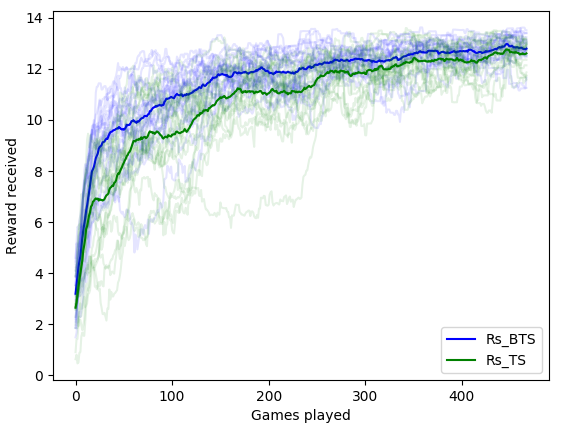
\includegraphics[width=0.7\textwidth,height=0.35\textheight]{../../pictures/figures/mab-9-ts.png}
  \caption{A 8 armed bandit problem, with means and variances chosen randomly.
	We can see that Biased Thompson sampling does not perform better in any significant sense.}
\end{figure}

\begin{figure}[h!]
  \centering
  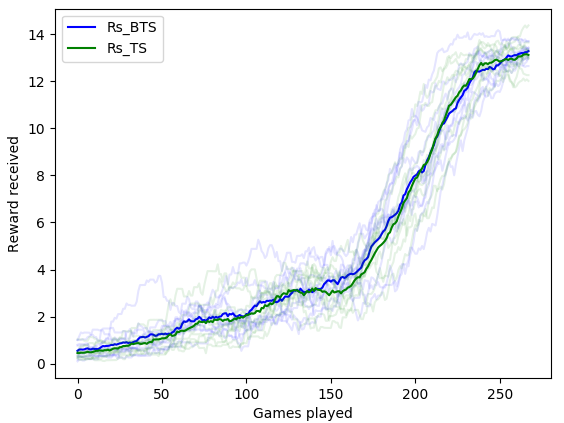
\includegraphics[width=0.7\textwidth,height=0.35\textheight]{../../pictures/figures/mdp-25-explicit.png}
  \caption{A 25 state XXX problem. With explicit knowledge of the underlying symmetry.
	We can see that Biased Thompson sampling does not perform better in any significant sense.}
\end{figure}

\begin{center}\rule{0.5\linewidth}{\linethickness}\end{center}

Of course, the symmetry didn't need to be inferred. So it's cheating.
We could have simply built the symmetry into the solver. But we want to
construct a 'high' level prior that is not specific to a single problem (like $S_2$ is), but
to many. Something that prefers symmetries of any kind.
